\begin{figure}[t]
\centering
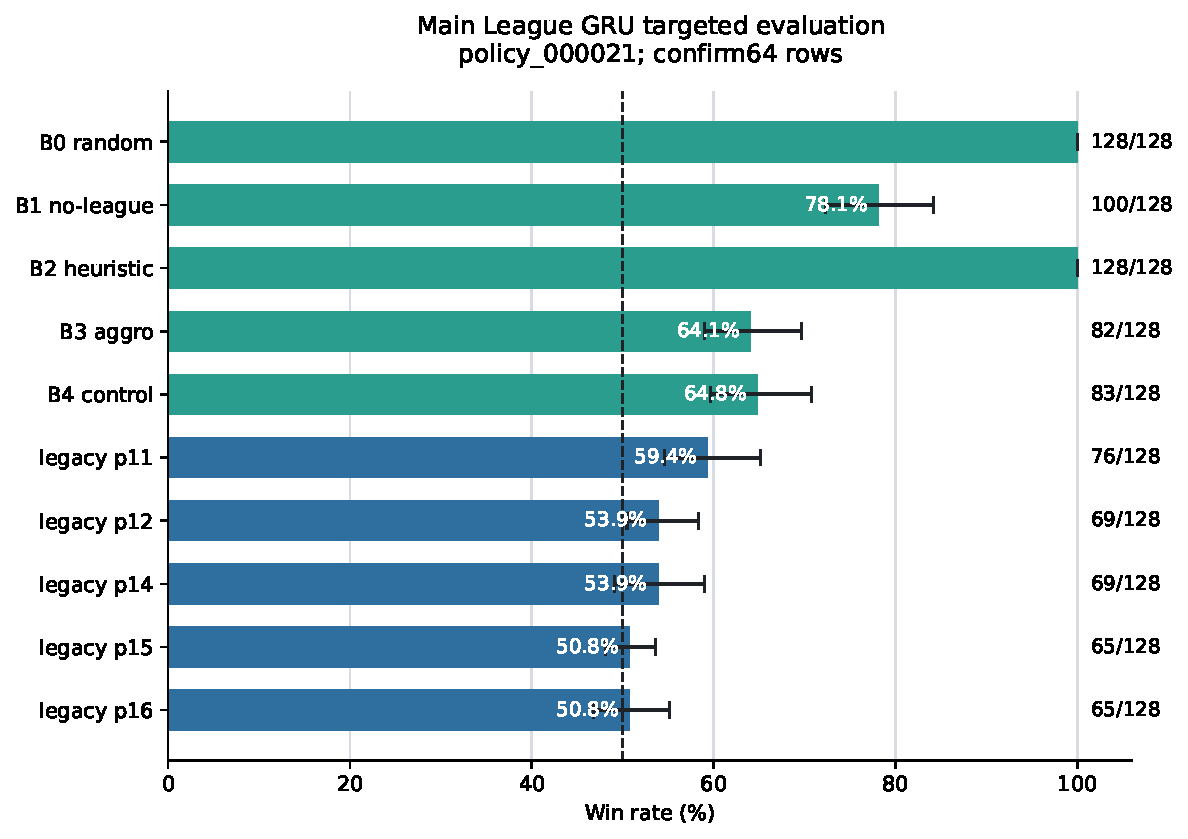
\includegraphics[width=\linewidth]{thesis_figures_final/fig_main_targeted_robustness.pdf}
\caption{Targeted confirm64 evaluation of the selected main League GRU policy against fixed anchors, corrected B3/B4 public heuristics, and legacy league snapshots. Error bars show bootstrap confidence intervals over paired seeds.}
\label{fig:main-targeted-robustness}
\end{figure}

\begin{table}[t]
\centering
\caption{Targeted evaluation of the selected main League GRU model, policy\_000021. All rows use 64 paired seeds (128 games) with seat-swapped evaluation.}
\label{tab:main-p21-targeted}
\begin{tabular}{lrrrr}
\toprule
Opponent & Wins & Games & Win rate & Issues \\
\midrule
B0 RandomLegal & 128 & 128 & 100.00\% & 0 \\
B1 NoLeague baseline & 100 & 128 & 78.12\% & 0 \\
B2 HeuristicPublic & 128 & 128 & 100.00\% & 0 \\
B3 HeuristicPublicAggro & 82 & 128 & 64.06\% & 0 \\
B4 HeuristicPublicControl & 83 & 128 & 64.84\% & 0 \\
Legacy p11 & 76 & 128 & 59.38\% & 0 \\
Legacy p12 & 69 & 128 & 53.91\% & 0 \\
Legacy p14 & 69 & 128 & 53.91\% & 0 \\
Legacy p15 & 65 & 128 & 50.78\% & 0 \\
Legacy p16 & 65 & 128 & 50.78\% & 0 \\
\bottomrule
\end{tabular}
\end{table}


\begin{figure}[t]
\centering
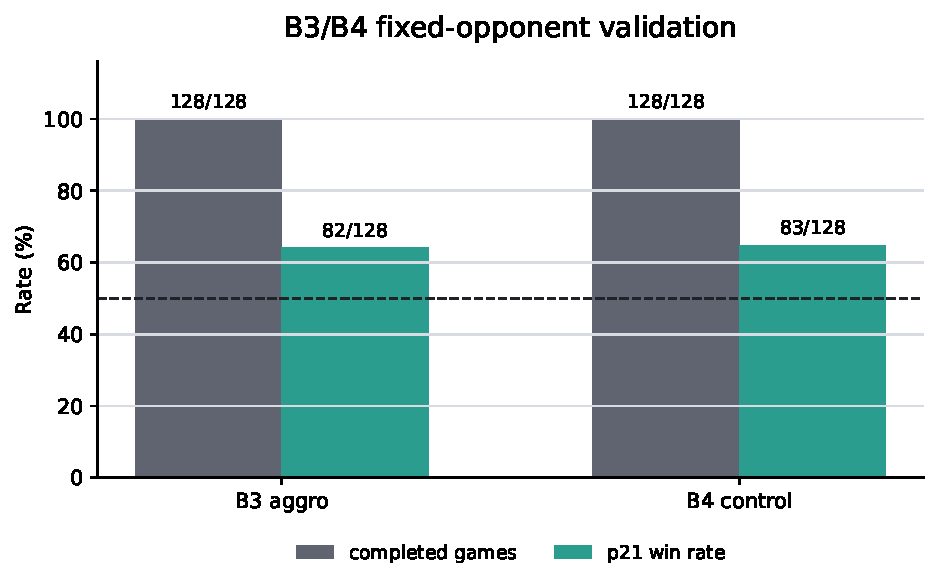
\includegraphics[width=0.82\linewidth]{thesis_figures_final/fig_b3b4_fixed_validation.pdf}
\caption{Validation of the corrected B3/B4 evaluation rows. The corrected aggressive/control heuristic opponents complete all games without truncation, and the selected policy remains above parity against both profiles.}
\label{fig:b3b4-fixed-validation}
\end{figure}

\begin{figure}[t]
\centering
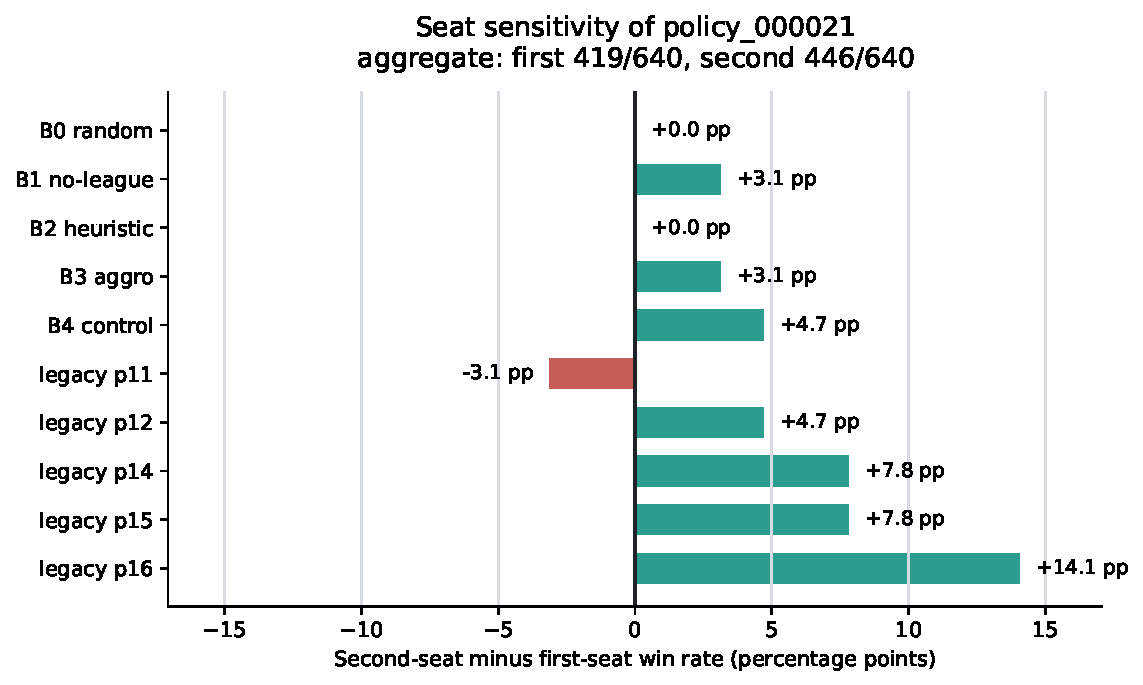
\includegraphics[width=0.82\linewidth]{thesis_figures_final/fig_p21_seat_advantage.pdf}
\caption{Seat sensitivity diagnostic for the targeted confirm64 table. Evaluations are paired and seat-swapped, so the measured first/second-seat asymmetry is diagnostic rather than a confound in the reported win rates.}
\label{fig:p21-seat-sensitivity}
\end{figure}

\begin{figure}[t]
\centering
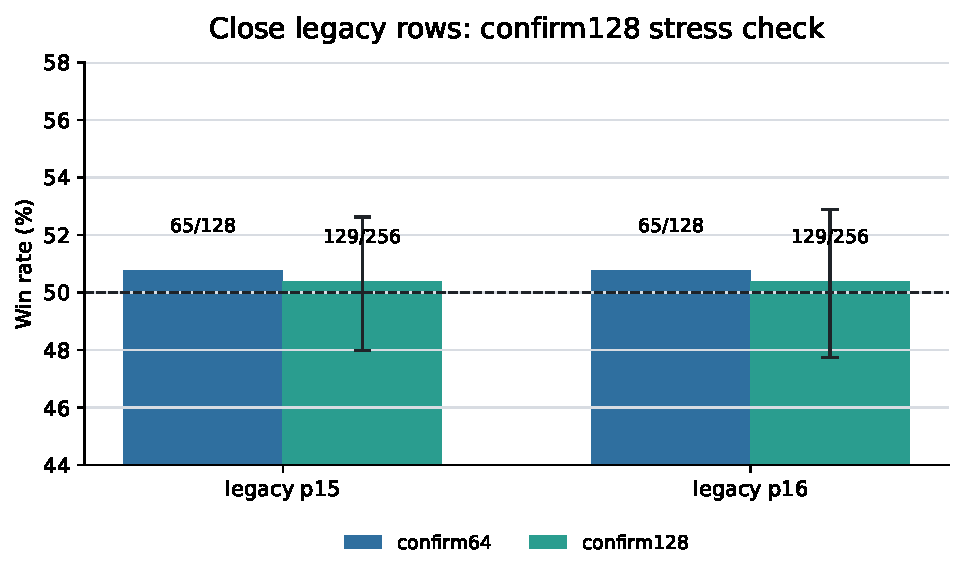
\includegraphics[width=0.72\linewidth]{thesis_figures_final/fig_close_legacy_stress.pdf}
\caption{Stress check for the two closest legacy neural rows. The rows remain slightly above parity at confirm128, but the margins are narrow and should be reported conservatively.}
\label{fig:close-legacy-stress}
\end{figure}

\begin{figure}[t]
\centering
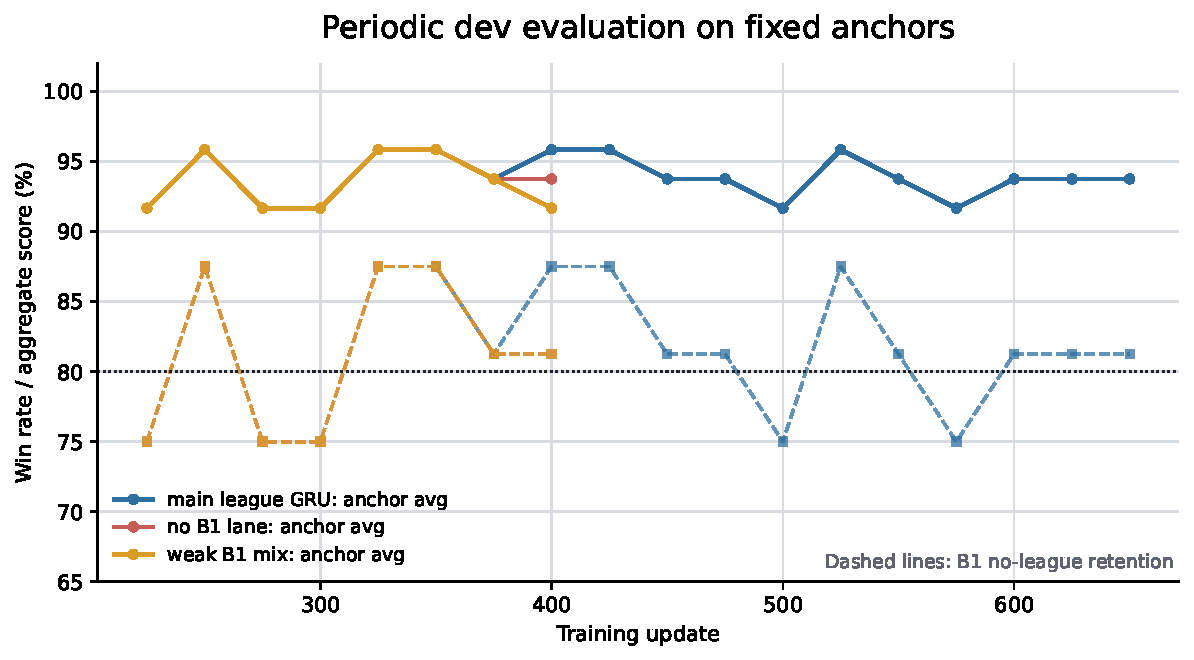
\includegraphics[width=0.88\linewidth]{thesis_figures_final/fig_anchor_retention.pdf}
\caption{Periodic development evaluation for the main model and B1-pressure ablations. Solid lines show aggregate anchor performance; dashed lines show B1 no-league retention.}
\label{fig:anchor-retention}
\end{figure}

\begin{figure}[t]
\centering
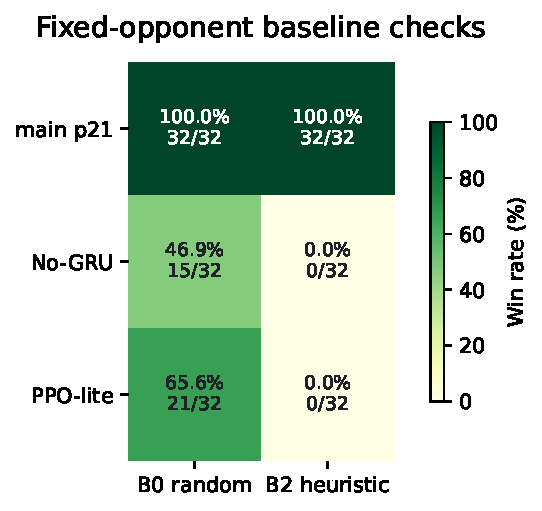
\includegraphics[width=0.72\linewidth]{thesis_figures_final/fig_baseline_fixed_grid.pdf}
\caption{Fixed-opponent baseline sanity checks. No-GRU and PPO-lite were not evaluated against the full B1/league opponent set, so this figure is a fixed-anchor baseline comparison rather than a full league-robustness comparison.}
\label{fig:fixed-baseline-grid}
\end{figure}
